\section{Aplicaciones de Machine Learning en la Maquiladora}\label{aplicaciones-de-machine-learning-en-la-maquiladora}

\subsection{\textbf{Introducción a Machine Learning (ML)}}\label{introduccion-a-machine-learning-ml}

El \textbf{Machine Learning} es una herramienta clave en el avance tecnológico de las maquiladoras. Aunque suena como un concepto complicado, en realidad es más sencillo de lo que parece: se trata de enseñar a las máquinas a \textbf{aprender} de los datos, tal como nosotros aprendemos de la experiencia. En lugar de programar una máquina para que haga exactamente lo que queremos (como en los sistemas tradicionales), \textbf{Machine Learning (ML)} permite que las máquinas identifiquen patrones, hagan predicciones y tomen decisiones basadas en esos datos.

Entonces, \textbf{¿por qué esto es importante para una maquiladora?} Porque la IA y el Machine Learning pueden ayudar a reducir errores, optimizar la producción, mejorar la calidad y anticipar problemas antes de que ocurran. Si tu línea de producción tiene un historial de fallas que cuesta tiempo y dinero, ¿no sería genial que una máquina te avisara antes de que suceda para que pudieras arreglarlo de antemano?

\begin{figure}[H]
\centering
\begin{adjustbox}{width=\textwidth}
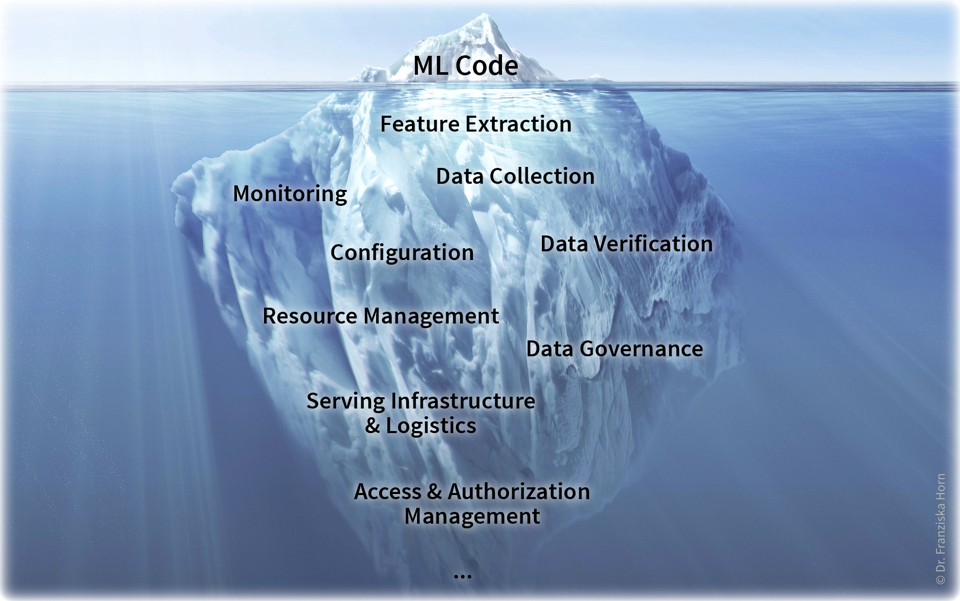
\includegraphics{img/imagen_186.jpg}
\end{adjustbox}
\caption{Meme sobre Machine Learning en la maquila}
\end{figure}

\section{\textbf{¿Qué es Machine Learning?}}\label{que-es-machine-learning}

El \textbf{Machine Learning} se basa en la idea de que una máquina puede aprender a hacer algo (como predecir fallas o mejorar un proceso) simplemente dándole acceso a muchos datos sobre ese algo. \textbf{Es como enseñar a alguien a resolver un problema dándole ejemplos de cómo se ha resuelto ese problema antes.}

Imagina que tienes datos sobre la producción de una máquina: las horas que opera, las temperaturas que alcanza, la cantidad de piezas que fabrica, etc. Si cada vez que la máquina fallaba también anotabas estas mismas características, podrías darle esos datos a un modelo de Machine Learning, y este aprendería a identificar las condiciones que llevan a una falla. \textbf{Básicamente, se trata de darle a la máquina un ``historial'' de lo que ha pasado, para que pueda predecir lo que pasará en el futuro}.

En resumen: \textbf{Machine Learning} es el arte de hacer que las máquinas aprendan de los datos, para que puedan tomar decisiones o hacer predicciones sin que les digas exactamente qué hacer en cada caso.

\begin{figure}[H]
\centering
\begin{adjustbox}{width=\textwidth}
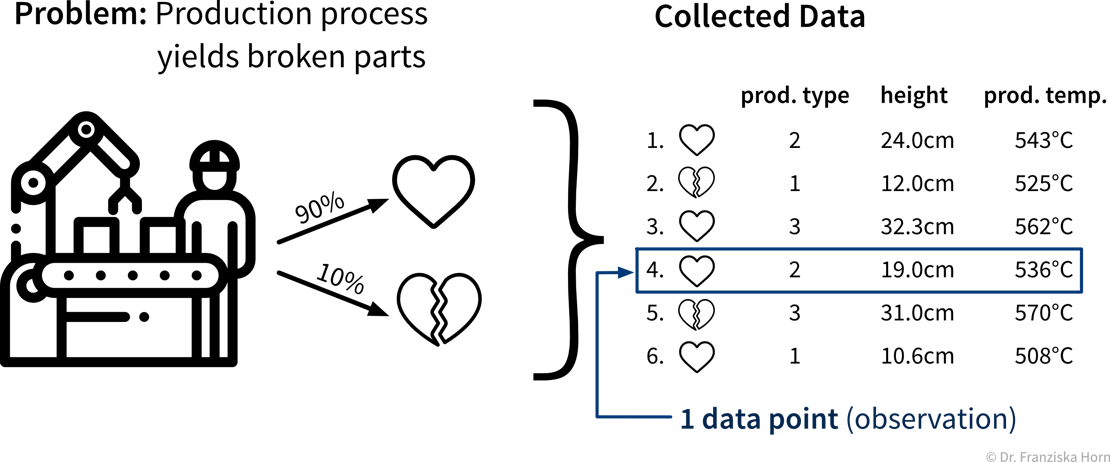
\includegraphics{img/imagen_32.jpg}
\end{adjustbox}
\caption{Meme sobre la predicción en Machine Learning}
\end{figure}

\subsubsection{\textbf{Aprendizaje Supervisado vs No Supervisado}}\label{aprendizaje-supervisado-vs-no-supervisado}

Existen dos tipos principales de Machine Learning, y entender la diferencia entre ellos te ayudará a identificar cuál es más útil en tu maquila.

\subsubsection{\textbf{Aprendizaje Supervisado}}\label{aprendizaje-supervisado}

El \textbf{aprendizaje supervisado} es como enseñarle a alguien a hacer algo mostrándole los ejemplos correctos y las respuestas. Le das a la máquina un conjunto de datos donde ya sabes lo que pasa (el resultado), y la máquina aprende a predecir ese resultado cuando vea datos nuevos.

\textbf{Ejemplo sencillo en la maquila}: Supón que tienes los datos de las máquinas en tu línea de producción y sabes qué condiciones llevaron a una falla (como vibraciones anormales o temperaturas extremas). Puedes entrenar a un modelo de Machine Learning para que, cuando vea esas mismas condiciones en una máquina en funcionamiento, te avise de que algo está mal antes de que ocurra una avería.

Este tipo de ML funciona muy bien cuando ya tienes información sobre lo que ha ocurrido y quieres predecir lo que sucederá en situaciones similares en el futuro.

\subsubsection{\textbf{Aprendizaje No Supervisado}}\label{aprendizaje-no-supervisado}

Por otro lado, el \textbf{aprendizaje no supervisado} es un poco más libre: es como darle un montón de información a la máquina y dejarla que descubra patrones por sí sola. No le dices qué debe buscar, simplemente la máquina agrupa los datos o encuentra similitudes entre ellos.

\textbf{Ejemplo sencillo en la maquila}: Digamos que tienes muchos datos sobre el rendimiento de tus máquinas, pero no sabes qué está afectando a la producción. Con el aprendizaje no supervisado, puedes descubrir patrones en los datos, como que ciertas máquinas siempre rinden menos a ciertas horas del día o cuando operan junto a otras máquinas específicas. La IA encontrará esos patrones, lo que te permitirá hacer ajustes en la producción que de otro modo no habrías notado.

\subsubsection{\textbf{El papel de ML en la maquila: ¿Por qué es importante?}}\label{el-papel-de-ml-en-la-maquila-por-que-es-importante}

Machine Learning puede transformar radicalmente la manera en que operas en la maquiladora. \textbf{¿Por qué?} Porque la IA no solo se trata de automatizar, sino de hacer más inteligentes las decisiones que tomas día a día.

\textbf{Imagina esto}: Tienes una línea de producción donde algunas máquinas fallan de vez en cuando. Esto significa paradas inesperadas, retrasos, y por supuesto, costos adicionales. Pero ¿qué pasaría si pudieras predecir cuándo esas máquinas van a fallar y hacer el mantenimiento antes de que ocurra la avería? Esto es lo que Machine Learning puede hacer por ti. Es como tener un ``sexto sentido'' en la producción.

Además, no solo hablamos de evitar fallas: Machine Learning puede ayudarte a ajustar el inventario de manera eficiente, prever la demanda, mejorar la calidad de los productos, y hasta optimizar la logística dentro de la planta. En resumen, \textbf{es una herramienta para ser más competitivo en un mercado que no para de moverse}.

\subsection{\textbf{Tipos de Machine Learning en la Maquila}}\label{tipos-de-machine-learning-en-la-maquila}

Ahora que ya tienes una idea básica de lo que es Machine Learning y por qué es tan relevante en la maquiladora, vamos a profundizar un poco más en los tipos de ML que puedes utilizar en tu planta. Dependiendo del tipo de problema que enfrentes, puedes elegir entre \textbf{aprendizaje supervisado} o \textbf{no supervisado}, e incluso otros enfoques como el \textbf{aprendizaje por refuerzo}.

\begin{figure}[H]
\centering
\begin{adjustbox}{width=\textwidth}
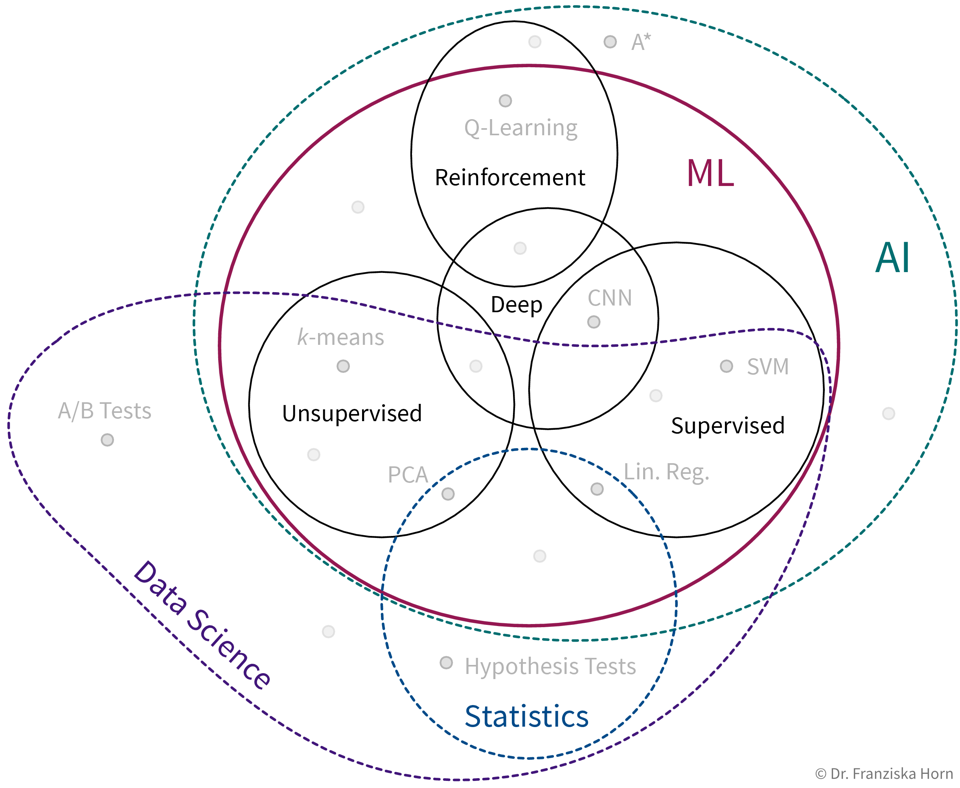
\includegraphics{img/imagen_21.jpg}
\end{adjustbox}
\caption{Meme sobre la importancia de elegir el tipo de Machine Learning}
\end{figure}

\subsubsection{\textbf{Aprendizaje Supervisado}}\label{aprendizaje-supervisado-1}

En el \textbf{aprendizaje supervisado}, el sistema aprende de datos que ya incluyen tanto las características (por ejemplo, temperatura de la máquina, tiempo de operación, etc.) como los resultados correctos (por ejemplo, si la máquina falló o no). Este tipo de aprendizaje es ideal cuando ya tienes un montón de información de tus procesos y quieres usarla para predecir futuros eventos.

\textbf{Ejemplo práctico}: Si sabes que ciertas condiciones en una máquina han llevado a su falla en el pasado, puedes entrenar un modelo de aprendizaje supervisado que prediga cuándo una máquina fallará de nuevo basándose en esas mismas condiciones. Esto es útil para el \textbf{mantenimiento predictivo}, que puede ahorrarte mucho tiempo y dinero.

\subsubsection{\textbf{Aprendizaje No Supervisado}}\label{aprendizaje-no-supervisado-1}

El \textbf{aprendizaje no supervisado} es como darle a la máquina una pila de datos y decirle ``¡descubre algo interesante!''. No le damos las respuestas de antemano, sino que la máquina encuentra patrones por su cuenta.

\textbf{Ejemplo práctico}: Puedes usar aprendizaje no supervisado para analizar datos de producción y descubrir relaciones que no habías visto antes. Por ejemplo, podrías descubrir que ciertas combinaciones de máquinas tienden a producir más errores en ciertos momentos del día. Este tipo de información es oro puro para optimizar la producción, ya que te permite tomar decisiones informadas basadas en lo que los datos te dicen, no en suposiciones.

\subsection{Conceptos Clave para Entender Machine Learning}\label{conceptos-clave-para-entender-machine-learning}

Para implementar \textbf{Machine Learning (ML)} de manera efectiva en una maquiladora, es fundamental comprender algunos conceptos clave que forman la base del aprendizaje automático. Estos términos te ayudarán a abordar los desafíos técnicos y a tomar decisiones más inteligentes a medida que avances en tu proceso de transformación digital.

\subsubsection{\textbf{Dataset: La Base de Todo}}\label{dataset-la-base-de-todo}

Un \textbf{dataset} es el conjunto de datos que alimenta al modelo de Machine Learning. \textbf{Piensa en el dataset como si fuera la materia prima de una maquiladora}, donde los datos son las piezas que la IA utiliza para aprender. Sin un buen dataset, el modelo no puede funcionar correctamente.

\textbf{Ejemplo en la maquila}: Supongamos que tienes datos históricos sobre las temperaturas de las máquinas, el tiempo que han estado operativas, el número de piezas que han producido y cuándo fallaron. Ese conjunto de datos es el ``dataset'' que alimentará tu modelo para que pueda aprender a predecir cuándo fallará una máquina en el futuro.

\subsubsection{\textbf{Variables Dependientes e Independientes}}\label{variables-dependientes-e-independientes}

En Machine Learning, las \textbf{variables} son los elementos de los datos que influyen en los resultados. Hay dos tipos de variables que debes conocer:

\begin{itemize}
    \item \textbf{Variables Independientes}: Son las entradas que proporcionan la información al modelo. Son como las características que describen un producto en una maquiladora. Por ejemplo, la temperatura de una máquina, la velocidad de producción o el número de horas trabajadas.
    \item \textbf{Variable Dependiente}: Es la salida o el resultado que estamos intentando predecir. Es lo que queremos que la máquina aprenda a identificar o calcular. En una maquiladora, la variable dependiente podría ser si una máquina va a fallar o no, o la cantidad de piezas defectuosas que produce una línea de producción.
\end{itemize}

\subsubsection{\textbf{Feature Engineering: La Clave del Éxito}}\label{feature-engineering-la-clave-del-exito}

El \textbf{feature engineering} es el proceso de elegir, transformar y crear las características (variables) que mejoran el rendimiento de un modelo de Machine Learning. Este paso es esencial porque no todas las variables son igual de útiles. Algunas variables pueden ser irrelevantes, mientras que otras pueden tener un impacto significativo en los resultados.

\subsubsection{\textbf{Preprocesamiento de Datos: Limpiando los Datos}}\label{preprocesamiento-de-datos-limpiando-los-datos}

El \textbf{preprocesamiento de datos} es uno de los pasos más importantes para que un modelo de Machine Learning funcione correctamente. Limpiarlos y prepararlos adecuadamente te permite sacar el máximo provecho de tu modelo de Machine Learning.

\subsection{\textbf{Ventajas del Machine Learning en la Maquiladora}}\label{ventajas-del-machine-learning-en-la-maquiladora}

El \textbf{Machine Learning} ofrece muchas ventajas para una maquiladora, desde la reducción de costos hasta la mejora en la eficiencia de los procesos. Aquí te detallamos las principales razones por las que integrar ML en tu maquila puede marcar la diferencia:

\subsubsection{\textbf{Rapidez en la Toma de Decisiones}}\label{rapidez-en-la-toma-de-decisiones}

Una de las mayores ventajas del Machine Learning es la \textbf{velocidad} con la que puede analizar grandes cantidades de datos y ofrecer resultados. Esto es especialmente útil en una maquiladora, donde la rapidez en la toma de decisiones puede marcar la diferencia entre cumplir con un pedido o retrasarse.

\subsubsection{\textbf{Facilidad de Uso y Sencillez}}\label{facilidad-de-uso-y-sencillez}

Hoy en día, las herramientas de Machine Learning son cada vez más accesibles, y muchas de ellas ofrecen interfaces simples que no requieren conocimientos avanzados en programación. Incluso si tu equipo no tiene experiencia con IA, \textbf{plataformas como AWS, Azure y Google Cloud} te permiten implementar modelos de manera sencilla y escalable.

\subsubsection{\textbf{Auditoría y Transparencia}}\label{auditoria-y-transparencia}

Otra ventaja clave es que \textbf{los modelos de Machine Learning pueden ser auditados}. Esto significa que puedes rastrear y verificar cómo el modelo llegó a una decisión o predicción, lo que es muy importante en industrias reguladas como la manufactura.

\subsection{\textbf{Desventajas del Machine Learning en la Maquiladora}}\label{desventajas-del-machine-learning-en-la-maquiladora}

Aunque \textbf{Machine Learning} tiene muchas ventajas, no es una solución mágica. Implementarlo también tiene desafíos y posibles desventajas que debes tener en cuenta.

\subsubsection{\textbf{Costo de Implementación}}\label{costo-de-implementacion}

A pesar de las ventajas a largo plazo, el costo inicial de implementar ML puede ser alto, especialmente si tu maquiladora no tiene ya la infraestructura necesaria.

\subsubsection{\textbf{Dudas Técnicas}}\label{dudas-tecnicas}

El éxito de un sistema de Machine Learning depende mucho de la calidad de los datos y del personal capacitado que pueda supervisar y ajustar los modelos.

\subsubsection{\textbf{Complejidad en el Análisis de Datos}}\label{complejidad-en-el-analisis-de-datos}

El análisis de datos en Machine Learning no es una tarea sencilla. Requiere tiempo y experiencia para preparar correctamente los datos, seleccionar las variables adecuadas y ajustar los modelos.

\subsection{\textbf{Conclusión de las Ventajas y Desventajas}}\label{conclusion-de-las-ventajas-y-desventajas}

En resumen, el \textbf{Machine Learning} tiene el potencial de revolucionar la maquiladora, optimizando procesos, reduciendo costos y mejorando la calidad de los productos. Sin embargo, la implementación tiene desafíos que deben considerarse cuidadosamente.

\subsection{\textbf{Referencias ML}}\label{referencias-ml}

\begin{enumerate}
    \item Russell, S. \& Norvig, P. \emph{Artificial Intelligence: A Modern Approach} (4th ed.). Prentice Hall, 2020.
    \item Goodfellow, I., Bengio, Y. \& Courville, A. \emph{Deep Learning}. MIT Press, 2016.
    \item Hastie, T., Tibshirani, R. \& Friedman, J. \emph{The Elements of Statistical Learning: Data Mining, Inference, and Prediction} (2nd ed.). Springer, 2009.
    \item Géron, A. \emph{Hands-On Machine Learning with Scikit-Learn, Keras, and TensorFlow} (2nd ed.). O'Reilly Media, 2019.
    \item Murphy, K. P. \emph{Machine Learning: A Probabilistic Perspective}. MIT Press, 2012.
    \item Bishop, C. M. \emph{Pattern Recognition and Machine Learning}. Springer, 2006.
\end{enumerate}

